\section{SPARQLed: Query Recommendation}
\label{sec:exploiting:sparqled:recommendation}

When a user formulates a SPARQL query, the user is in fact trying to summarise his information needs. However, this task can be very difficult and time consuming as it requires the user to have a good knowledge of the structure and vocabulary of the dataset he is trying to query. This task becomes even more complex if the user is trying to formulate a query across multiple data sources. In order to gain such knowledge, the user must explore and investigate the data itself before querying it.

To save the user from such a tedious work we present the \emph{Assisted SPARQL Editor}, an application that leverages the graph summary to help the user into effectively formulating complex SPARQL queries, even without prior knowledge about the structure and vocabulary of the data sources.\\

In this section, we first give an overview of the possible recommendations supported by the SPARQL editor, and then, we introduce some of the main concepts in SPARQL. The summary is RDFied using the model presented in Section~\ref{chap03:sec:wd-mgnt} so that it can be queried: we describe how the current state of the SPARQL query is used to query the graph summary. The \emph{Full} reification of the summary is used. The results from the summary are then recommended to the user as possible structural query elements.

\subsection{Overview of SPARQL Recommendations}

The Assisted SPARQL Editor supports four kinds of recommendations: class, predicate, relationships between variables and named graphs. Examples of such recommendations are pictured in Figures~\ref{fig:rkb-recommendations}. Recommendations of entity node labels as well as literal node labels are not supported since such content data is discarded from the graph summary.

During query formulation, the assisted editor provides one of these four different types of recommendations to the user based on the state of the edited query. The state of the edited query is composed of an incomplete graph pattern and the cursor position. The cursor position materialises the \gls{POF}, i.e., the unknown element of the graph pattern for which the user requests recommendations. The \gls{POF} is depicted in Figures~\ref{fig:rkb-recommendations} with an angle bracket.

\paragraph{Class recommendation.}

Figure~\ref{fig:rkb-recommendations-types} depicts the recommendations of possible classes for a variable. Given that the variable \emph{?Article} is associated to a predicate \emph{akt:hasAuthor}, the system will only recommend classes that are mentioned with this predicate in the graph.

\paragraph{Predicate recommendation.}

Figure~\ref{fig:rkb-recommendations-predicates} depicts the recommendation of additional predicates for the class \emph{akt:Article-Reference} which co-occur with the property \emph{akt:hasAuthor}.
%In the case of class recommendation, elements of the node collection labels are retrieved from the graph summary and presented as possible recommendations.
%In the case of predicate recommendation, c-linkset labels $\mathcal{L}^A$ are retrieved from the graph summary and presented to the user.

\paragraph{Relationships recommendation.}

Figure~\ref{fig:rkb-recommendations-relations} depicts recommendations of possible relationships between two variables. The only predicates that are returned as a recommendation are those that connect an author to an organisation.
%The current implementation of the Assisted SPARQL Editor only supports direct relationships, but in future work we expect to provide recommendations about possible shortest paths between two variables.

\paragraph{Named graph recommendation.}

In Figure~\ref{fig:rkb-recommendations-graph}, possible named graphs are recommended to the user. The proposed named graphs are those that contain at least one solution for the graph pattern.
%In this case, dataset labels $\mathcal{L}^D$ are retrieved from the graph summary.

\begin{figure}
	\centering
	\begin{subfigure}[t]{.475\textwidth}
		\resizebox{\textwidth}{!}{
			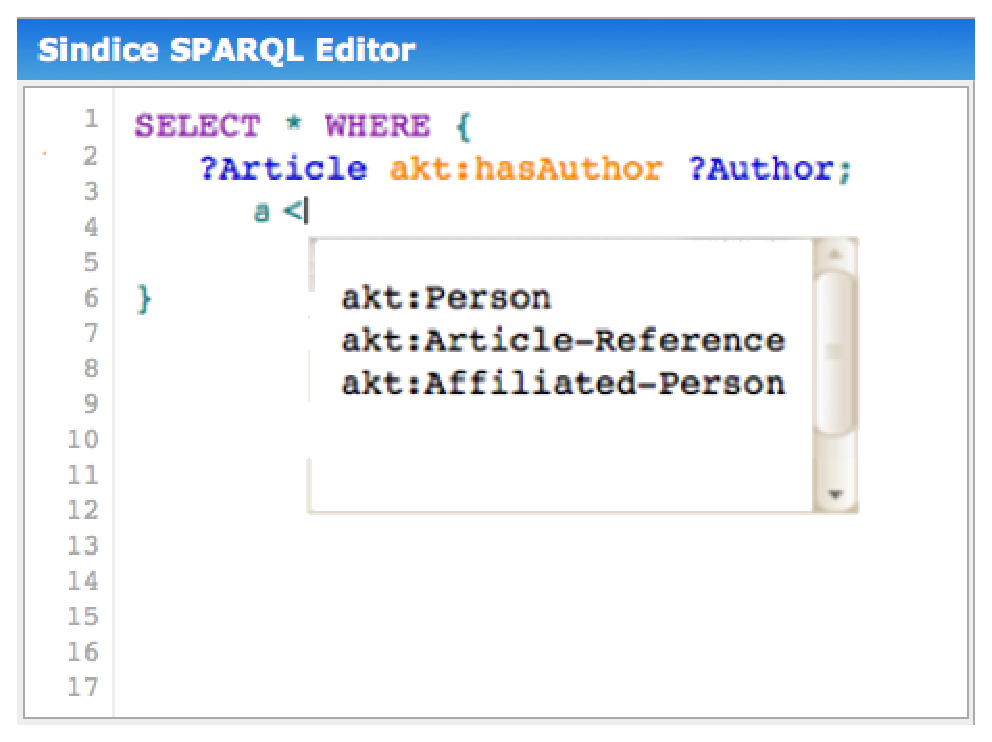
\includegraphics[scale=1]{07-systems/sparqled/figures/sparql/demo1.eps}
		}
		\caption{Class}
		\label{fig:rkb-recommendations-types}
	\end{subfigure}
	\begin{subfigure}[t]{.475\textwidth}
		\resizebox{\textwidth}{!}{
			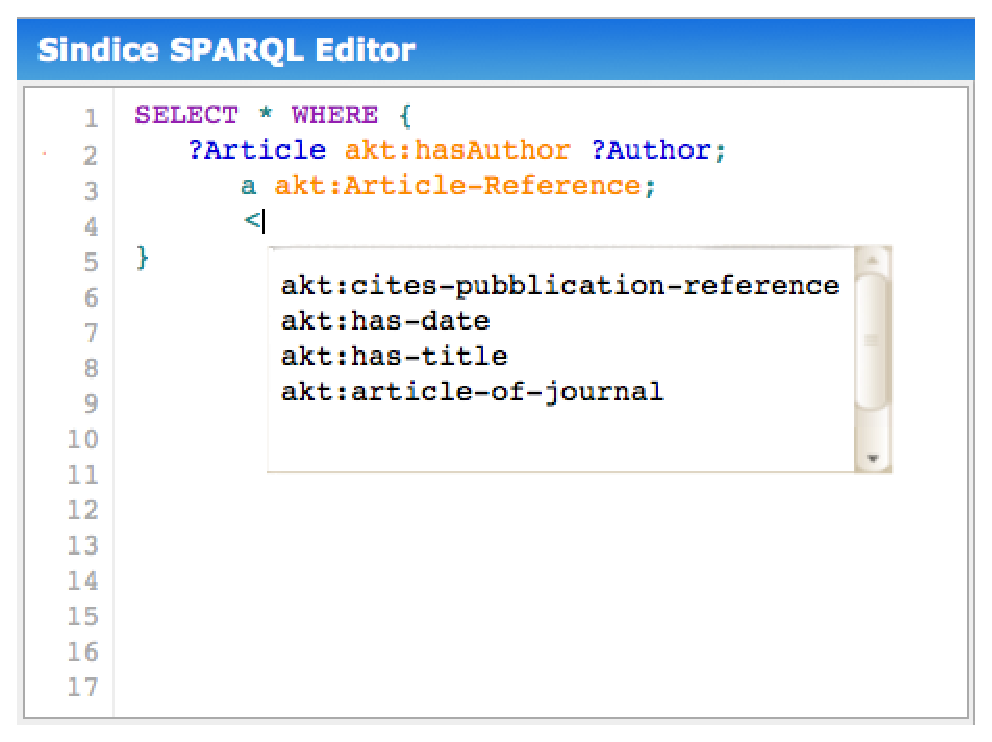
\includegraphics[scale=1]{07-systems/sparqled/figures/sparql/demo2.eps}
		}
		\caption{Predicate}
		\label{fig:rkb-recommendations-predicates}
	\end{subfigure}
	\qquad
	\begin{subfigure}[b]{.475\textwidth}
		\resizebox{\textwidth}{!}{
			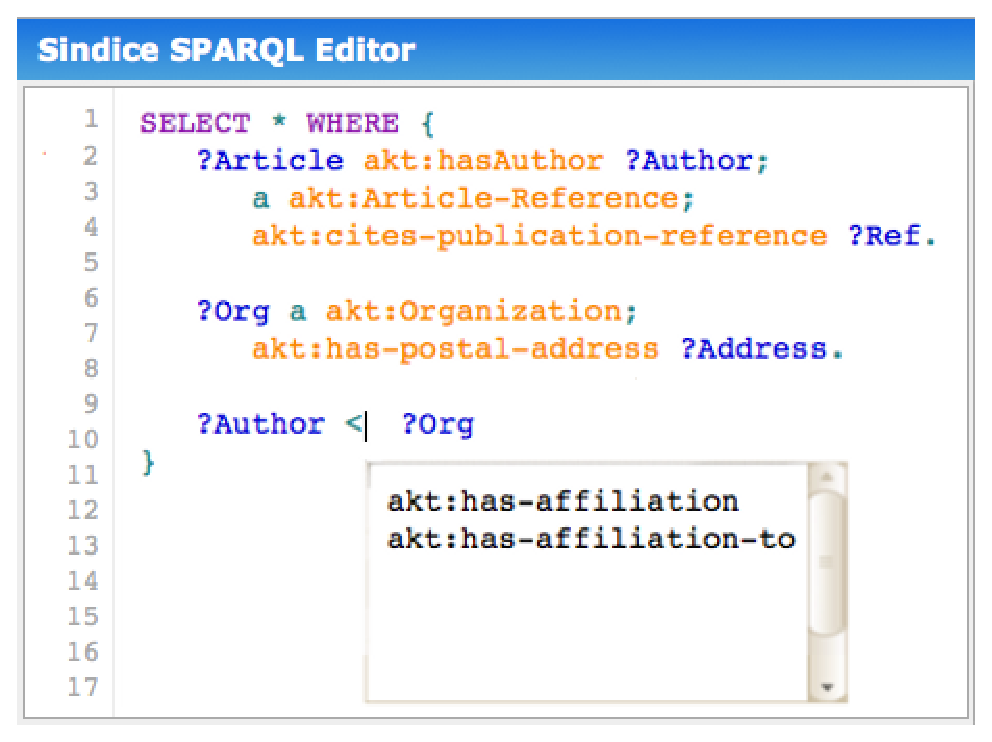
\includegraphics[scale=1]{07-systems/sparqled/figures/sparql/demo3.eps}
		}
		\caption{Relationships}
		\label{fig:rkb-recommendations-relations}
	\end{subfigure}
	\begin{subfigure}[b]{.475\textwidth}
		\resizebox{\textwidth}{!}{
			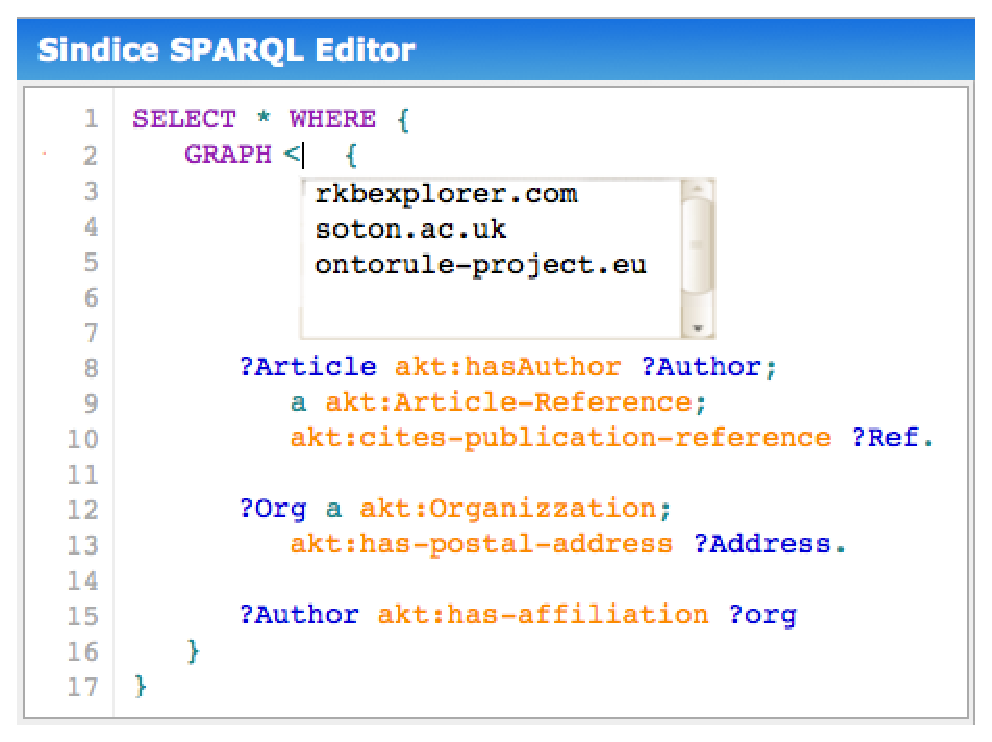
\includegraphics[scale=1]{07-systems/sparqled/figures/sparql/demo4.eps}
		}
		\caption{Named Graphs}
		\label{fig:rkb-recommendations-graph}
	\end{subfigure}
	\caption[Overview of possible recommendations in SPARQLed]{Overview of the possible recommendations for the \url{http://www.rkbexplorer.com} dataset depending on the Point of Focus. The Point of Focus is displayed by the green angle bracket $<$.}
	\label{fig:rkb-recommendations}
\end{figure}

\subsection{SPARQL Graph Pattern}

In this section, we introduce the main concepts of SPARQL that are used later in the description of our recommendation engine. SPARQL is the standard query language for RDF data and is based around graph pattern matching. Triple Pattern described in Definition~(\ref{def:triple-pattern}) is the building block in SPARQL.

Triple patterns can be combined into a Basic Graph Pattern (BGP)~\cite{PrudS08}. More complex graph patterns can be formed by combining BGPs in different ways~\cite{PrudS08}: \emph{Group Graph Pattern}, \emph{Optional Graph Pattern}, \emph{Alternative Graph Pattern} and \emph{Patterns on Named Graphs}.\\

A SPARQL query can be translated into an Abstract Syntax Tree (AST). The AST is a tree structure composed of all the logical operators of the query and where leaf nodes are triple patterns to be evaluated. Such an AST is the data structure used by our system to translate the current user need into possible recommendations. In our implementation, the AST may contain no more than one incomplete triple pattern and a special symbol `$<$' to indicate the \emph{Point of Focus}. A triple pattern is incomplete if all three components are not present.

\subsection{Definitions}

We introduce in this section definitions that are needed for describing our approach for SPARQL query recommendation.

Similar to triple patterns in SPARQL, summary patterns are the building blocks to construct a graph summary query.

\begin{definition}[Summary Pattern]
	Let $G=\left\langle V, A, l_V \right\rangle$ be a graph, $\mathcal{S} = \left\langle \mathcal{W}, \mathcal{B}, l_{\mathcal{W}} \right\rangle$ be the summary of $G$, and $\mathcal{L}$ be the set of labels, and $Var$ an infinite set of variables.

	A \emph{summary pattern} is a tuple $t = \langle s, p, o \rangle$ where $t \in (\mathcal{L} \cup Var) \times (\mathcal{L} \cup Var) \times (\mathcal{L} \cup Var)$.
	A sumedge $(x,\alpha,y) \in \mathcal{B}$ of the summary $\mathcal{S}$ is a match for a summary pattern $t$ if and only if the non-variable components of $t$ are equal to those of the sumedge $(x, \alpha, y)$.
	\label{def:summary-triple-pattern}
\end{definition}

We call \emph{class triple pattern} (CTP) a triple pattern which predicate is a type attribute (Section~\ref{sec:ssd:type}).

\begin{definition}[Class Triple Pattern]
	Let $G=\left\langle V, A, l_V \right\rangle$ be a graph, $\mathcal{L}$ be the set of labels, and $Var$ an infinite set of variables.
	A class triple pattern (CTP) is a triple $t= \langle s, \glssymbol{atype}, o \rangle$ where $t \in (\mathcal{L} \cup Var) \times T \times (\mathcal{L} \cup Var)$ where $predicate(t)$ is a type attribute.
	\label{def:class-triple-pattern}
\end{definition}

Similarly to triple patterns, summary patterns may be used to build more complex pattern, such as BGPs, as described in the previous section.

\subsection{From Entity Graph to Graph Summary}

In order to suggest the possible structural elements to the user with respect to the current state of his query, we need to \emph{normalise} the AST of the query to match the RDF data model of the summary introduced in Section~\ref{chap03:sec:wd-mgnt}. The normalised AST is then evaluated on the graph summary and the possible structural elements are retrieved and presented to the user.

The AST normalisation is performed in three steps:
\begin{enumerate}
	\item transformation of the \gls{POF} symbol `$<$' into a variable to project as the query solution;
	\item removal of content elements from the AST; and
	\item mapping of triple patterns into \emph{summary patterns}.
\end{enumerate}
Each step is part of the normalisation sequence: an operation is performed on a step, which result becomes then the input of the next step.
In the following section we describe in detail the normalisation of a SPARQL query.

\subsubsection{Abstract Syntax Tree Normalisation}

In this section, we describe the algorithm for normalising the AST of a SPARQL query into another AST that can be executed over a graph summary.
We illustrate each step thanks to the following SPARQL query over a fictional entity graph:

\begin{minted}[linenos,frame=lines,framesep=1mm]{sparql}
ASK WHERE {
  :article1 a :Article ;
            :title ?t .
 
  ?i a :Institute ;
     :employs ?p .
 
  ?p :name "Renaud" ;
     <                  # POF
}
\end{minted}

\paragraph{Step 1 --- \emph{Projection of the POF}.}

The first step consists in defining the variable to project as the query solution. In the triple pattern containing the \gls{POF}, we transform the \gls{POF} symbol into a variable $?POF$ and complete that triple pattern with a wildcard variable if needed. We denote as a wildcard variable a variable that is unique in the query. The initial \emph{Query Form}~\cite{PrudS08} of the AST is replaced by a projection of the \gls{POF} variable using the \emph{SELECT} form.

For example in the ongoing SPARQL query, the \gls{POF} symbol `$<$' at line 9 is translated into the variable $?POF$, and the wildcard variable $?\_z2$ is added to complete that triple pattern.
 The result of that step on the query is depicted below:

\begin{minted}[linenos,frame=lines,framesep=1mm]{sparql}
SELECT ?POF WHERE {     # Projection of the POF
  :article1 a :Article ;
            :title ?t .
 
  ?i a :Institute ;
     :employs ?p .
 
  ?p :name "Renaud" ;
     ?POF ?_z2           # Materialisation of the POF
}
\end{minted}

\paragraph{Step 2 --- \emph{Removal of content elements}.}

The second step consists in removing all content elements from the AST. A content element is an element that describes a specific aspect of an entity --- thus it does not inform about its structure.

Literals and URIs that appear in a triple pattern at a subject or object position are replaced with a wildcard variable.
For instance, the literal ``Renaud'' in line~8 is replaced by the variable $?\_z1$ in the SPARQL query below.

If the triple pattern is a CTP, then only the element at the subject position is replaced with a wildcard variable.
The triple pattern on line~2 of the ongoing SPARQL example is a CTP. Therefore, the object URI is left as is, but the subject URI \emph{:article1} is replaced with the variable $?\_z0$.

\begin{minted}[linenos,frame=lines,framesep=1mm]{sparql}
SELECT ?POF WHERE {
  ?_z0 a :Article ;      # The variable ?_z0 replaces the URI :article1
       :title ?t .
 
  ?i a :Institute ;
     :employs ?p .
 
  ?p :name ?_z1 ;        # The variable ?_z1 replaces the literal "Renaud"
     ?POF ?_z2
}
\end{minted}

\paragraph{Step 3 --- \emph{Mapping}.}

The third step consists of mapping each triple pattern to a summary pattern according to the following two rules.
The RDF data model of the summary this operation maps to is described in Section~\ref{chap03:sec:wd-mgnt}.

\begin{enumerate}
	\item If the triple pattern $\langle ?s,\; p,\; o \rangle$ is a CTP, then it is replaced with the following BGP:
	\begin{enumerate}
		\item A triple pattern $\langle ?s,\; \text{:feature},\; \text{\_:b0} \rangle$ is created in order to describe the CTP;
		\item A triple pattern $\langle \text{\_:b0},\;\text{:label},\; o \rangle$ is created to set the label of the type, e.g., \emph{:Article}; and
		\item A triple pattern $\langle \text{\_:b0},\;\text{:type},\; p \rangle$ is created to set the label of the type attribute, e.g., \emph{rdf:type}.
	\end{enumerate}
\item Otherwise, the triple pattern \mbox{$\langle ?s, p, ?o \rangle$} is replaced with the following BGP. We remark that in this case, both subject and object elements are variables due to the previous step.
	\begin{enumerate}
		\item A new wildcard variable $?x$ representing a sumedge $x$ is created;
		\item A triple pattern $\langle ?x,\; \text{:source},\; ?s \rangle$ is created to set the source of the sumedge;
		\item A triple pattern $\langle ?x,\; \text{:target},\; ?o \rangle$ is created to set the target of the sumedge; and
		\item A triple pattern $\langle ?x,\; \text{:label},\; p \rangle$ is created to set the label of the sumedge.
	\end{enumerate}
\end{enumerate}

For example, if we apply these mapping rules on the ongoing SPARQL query, the first triple pattern \mbox{$\langle ?\_z0, a, Article \rangle$} is translated into the summary pattern displayed on line~3 below since it is a CTP. The second triple pattern \mbox{$\langle ?\_z0, :title, ?t \rangle$} is translated into the BGP on line~5 of the query below.

\begin{minted}[linenos,frame=lines,framesep=1mm]{sparql}
SELECT ?POF WHERE {
  # Mapping of the triple pattern ?_z0 a :Article
  ?_z0 :feature [ :label :Article ; :type rdf:type ] .
  # Mapping of the triple pattern ?_z0 :title ?t
  ?se0 :source ?_z0; :target ?t; :label :title .
 
  # Mapping of the triple pattern ?i a :Institute
  ?i :feature [ :label :Institute ; :type rdf:type ] .
  # Mapping of the triple pattern ?i :employs ?p
  ?se1 :source ?i; :target ?p; :label :employs .
 
  # Mapping of the triple pattern ?p :name ?_z1
  ?se2 :source ?p; :target ?_z1; :label :name .
  # Mapping of the triple pattern ?p ?POF ?_z2
  ?se3 :source ?p; :target ?_z2; :label ?POF .
}
\end{minted}

\subparagraph{Graph graph pattern.}

A \emph{Graph Graph Pattern}~\cite{PrudS08} is an operator in SPARQL that indicates which dataset the associated graph patterns should be queried on. For example, in the SPARQL query below the first triple pattern is queried against the dataset \emph{:dbpedia}. In the second graph graph pattern, the user seeks recommendations on the possible datasets where the triple pattern ``\emph{?movie :title "Terminator"}'' might occur in.

\begin{minted}[linenos,frame=lines,framesep=1mm]{sparql}
SELECT * WHERE {
  GRAPH :dbpedia {
    ?character :name "John Connor"
  }
  GRAPH < {
    ?movie :title "Terminator"
  }
}
\end{minted}

We need to retain the desired dataset thanks to the vocabulary term \emph{:origin} in order to provide correct recommendations to the user. The query above is then normalised to the query below:

\begin{minted}[linenos,frame=lines,framesep=1mm]{sparql}
SELECT ?POF WHERE {
  # Mapping of the first graph graph pattern
  ?se0 :source ?character; :target ?_z0; :label :name, :origin :dbpedia .
  # Mapping of the second graph graph pattern
  ?se1 :source ?movie; :target ?_z1; :label :title, :origin ?POF .
}
\end{minted}

\subsection{User Interaction}

The purpose of the Assisted SPARQL query editor is to assist a user in writing a query. Therefore, there is a need to consider how the user interacts with the application.
In this section, we present two angles into improving the interaction. First, we discuss the ranking of recommendations. Next, we introduce the notion of scope for a recommendation.

\subsubsection{Recommendation Ranking}

In Section~\ref{sec:summary-ranking}, we discussed the ranking of solutions to a SPARQL query executed on a graph summary. For the purpose of improving the user interaction, it is possible to rank the recommendations using the \gls{MF} ranking model. As reported by the experiment in Section~\ref{sec:summary-ranking:eval}, the \gls{MF} model provides noticeable benefits over a simple ranking.

Applying the \gls{MF} model to rank recommendations allow us to present first to the user the recommendations that are most likely not part of the error set. Thus, we reduce the chances of a user to be frustrated over a recommendation that yields no result.

\subsubsection{Recommendation Scope}

During the formulation of a query, the query may contain multiple BGPs where some do not return any results. The system will therefore no longer produce recommendations, as the evaluation of the graph summary query will also not produce any results. However, this can be interpreted incorrectly by the user since he might believe that the dataset does not contain any other information. In order to minimise this issue, we introduce the notion of \emph{recommendation scope}.\\

The \emph{recommendation scope} helps to reduce the extent of the area that is relevant for the recommendation. Instead of taking into account the full SPARQL query, the recommendation engine will take only a relevant subset.

The recommendation scope is defined recursively by including all the triple patterns with a path to the \gls{POF} variable. A \emph{breadth-first search} algorithm on the query, starting on the POF node, is performed in order to find all the graph components that are connected to the POF. All the graph components that are not connected to the \gls{POF} are removed. This prevents non-relevant (to the \gls{POF}) triple patterns from limiting the recommendations.

For example, we take the SPARQL query that we used as illustration in the previous section.

\begin{minted}[linenos,frame=lines,framesep=1mm]{sparql}
ASK WHERE {
  :article1 a :Article ; :title ?t .
  ?i a :Institute ; :employs ?p .
  ?p :name "Renaud" ; <
}
\end{minted}

The first BGP on line~2 is not connected to the BGP that contains the \gls{POF} on line~4. Indeed, neither the URI \emph{:article1} nor the variable \emph{?t} are referenced in the other two BGPs. Therefore, that first BGP is outside of the recommendation scope. After normalising the SPARQL query, we remove that BGP from the query to be run on the graph summary, as depicted below:

\begin{minted}[linenos,frame=lines,framesep=1mm]{sparql}
SELECT ?POF WHERE {
  # Mapping of the triple pattern ?i a :Institute
  ?i :feature [
    :label :Institute ;
    :type rdf:type
  ] .
  # Mapping of the triple pattern ?i :employs ?p
  ?se1 :source ?i;
       :target ?p;
       :label :employs .
 
  # Mapping of the triple pattern ?p :name ?_z1
  ?se2 :source ?p;
       :target ?_z1;
       :label :name .
  # Mapping of the triple pattern ?p ?POF ?_z2
  ?se3 :source ?p;
       :target ?_z2;
       :label ?POF .
}
\end{minted}

%Another possible solution for this issue is to provide to the user an estimation of the cardinality of TPs or BGPs that can lead to an empty result set. This is possible given the cardinality information provided by the graph summary. We are currently planning to investigate this solution for future works.

%\subsection{Entity Authority}
%\todo{move this to the applications part}

%When working with the Web of Data, it is legitimate to wonder about the quality of the data. The quality not according to whether the data follows modelling standards or not, but rather to the information itself. Indeed, in an environment where data can be edited by anybody, it can happen that some statements about an entity, or relationships between two entities, can be erroneous. Therefore, there is a need to define the \emph{authority} of an entity in order to judge how much confidence one can put in the information about the entity that a dataset provides.\todo{Define the dataset set}

%\begin{definition}[Entity Authority]
%Let $v \in V$ an entity and $a_v : V \mapsto \mathcal{L}^D$ a function which assigns a dataset label to an entity, called the entity \emph{authority}. Statements about an entity are then said \emph{authoritative} if the dataset label given by $a_v$ and the label of the dataset where the statements are found are the same.
%\end{definition}

%For example, the authority of an entity is \emph{D1}, but a statement about that entity is found in a dataset labelled \emph{D2}; the validity of that statement should then be checked.
